\chapter{One-shot Detail Retouching}
\label{one-shot-add}
Table \ref{tablecomparison} compares the proposed detail retouching technique with a U-Net model\cite{ronneberger2015u}, ASAPNet generator \cite{shaham2021spatially}, and Deep edge-aware filters \cite{xu2015deep} over 182 images (100 face images, 22 material images, 30 room images, and 30 landscape images) across four different image processing filters (Gaussian, unsharp masking, bilateral filtering and \gls{LLF}). Below, additional qualitative comparison results from the calculation of Table \ref{tablecomparison} can be found. Note that bilater


\begin{figure}[ht]
  \centering
  % \fbox{\rule{0pt}{2in} \rule{0.9\linewidth}{0pt}}
    %\adjustbox{trim={0.0\width} {.62\height} {0.0\width} {0.0\height},clip}%
  {`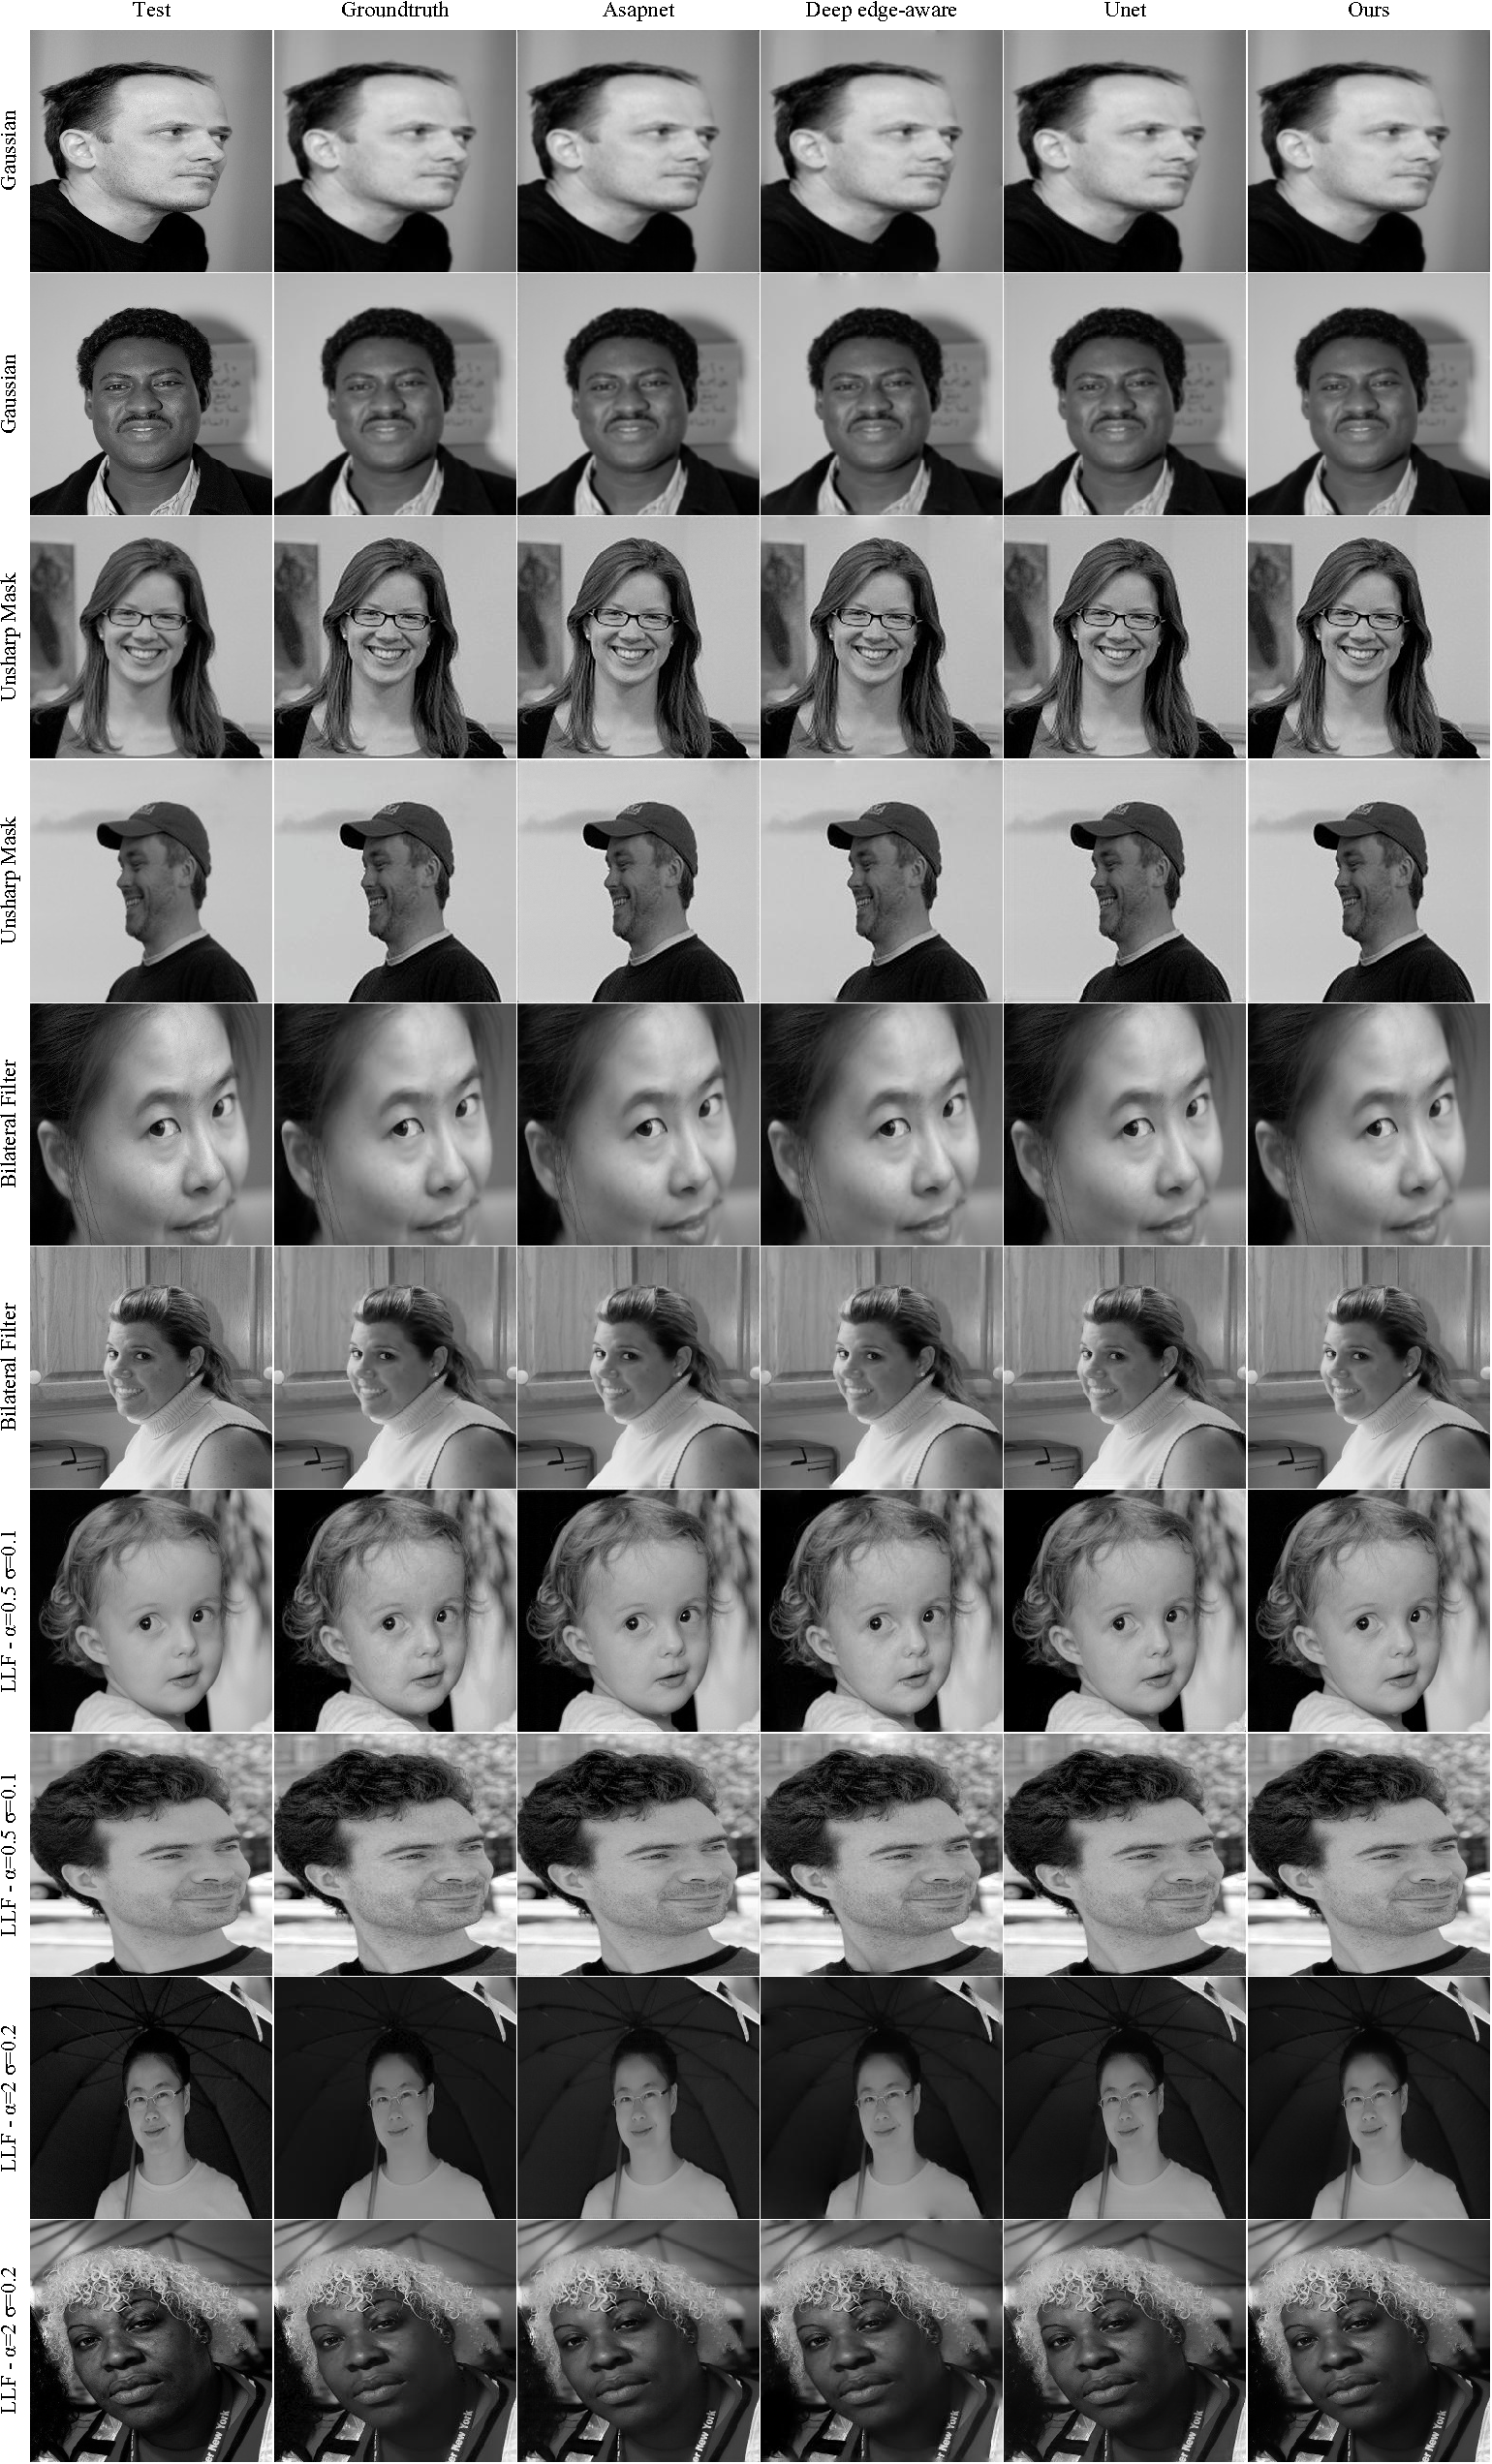
\includegraphics[width=0.8\linewidth]{Chapters/appendix-figs/face.pdf}}

   \caption{Qualitative comparison - Additional results.}
   \label{fig:appendix-DR-face}
\end{figure}

\begin{figure}[ht]
  \centering
  % \fbox{\rule{0pt}{2in} \rule{0.9\linewidth}{0pt}}

    %\adjustbox{trim={0.0\width} {.\height} {0.0\width} {0.385\height},clip}%
  {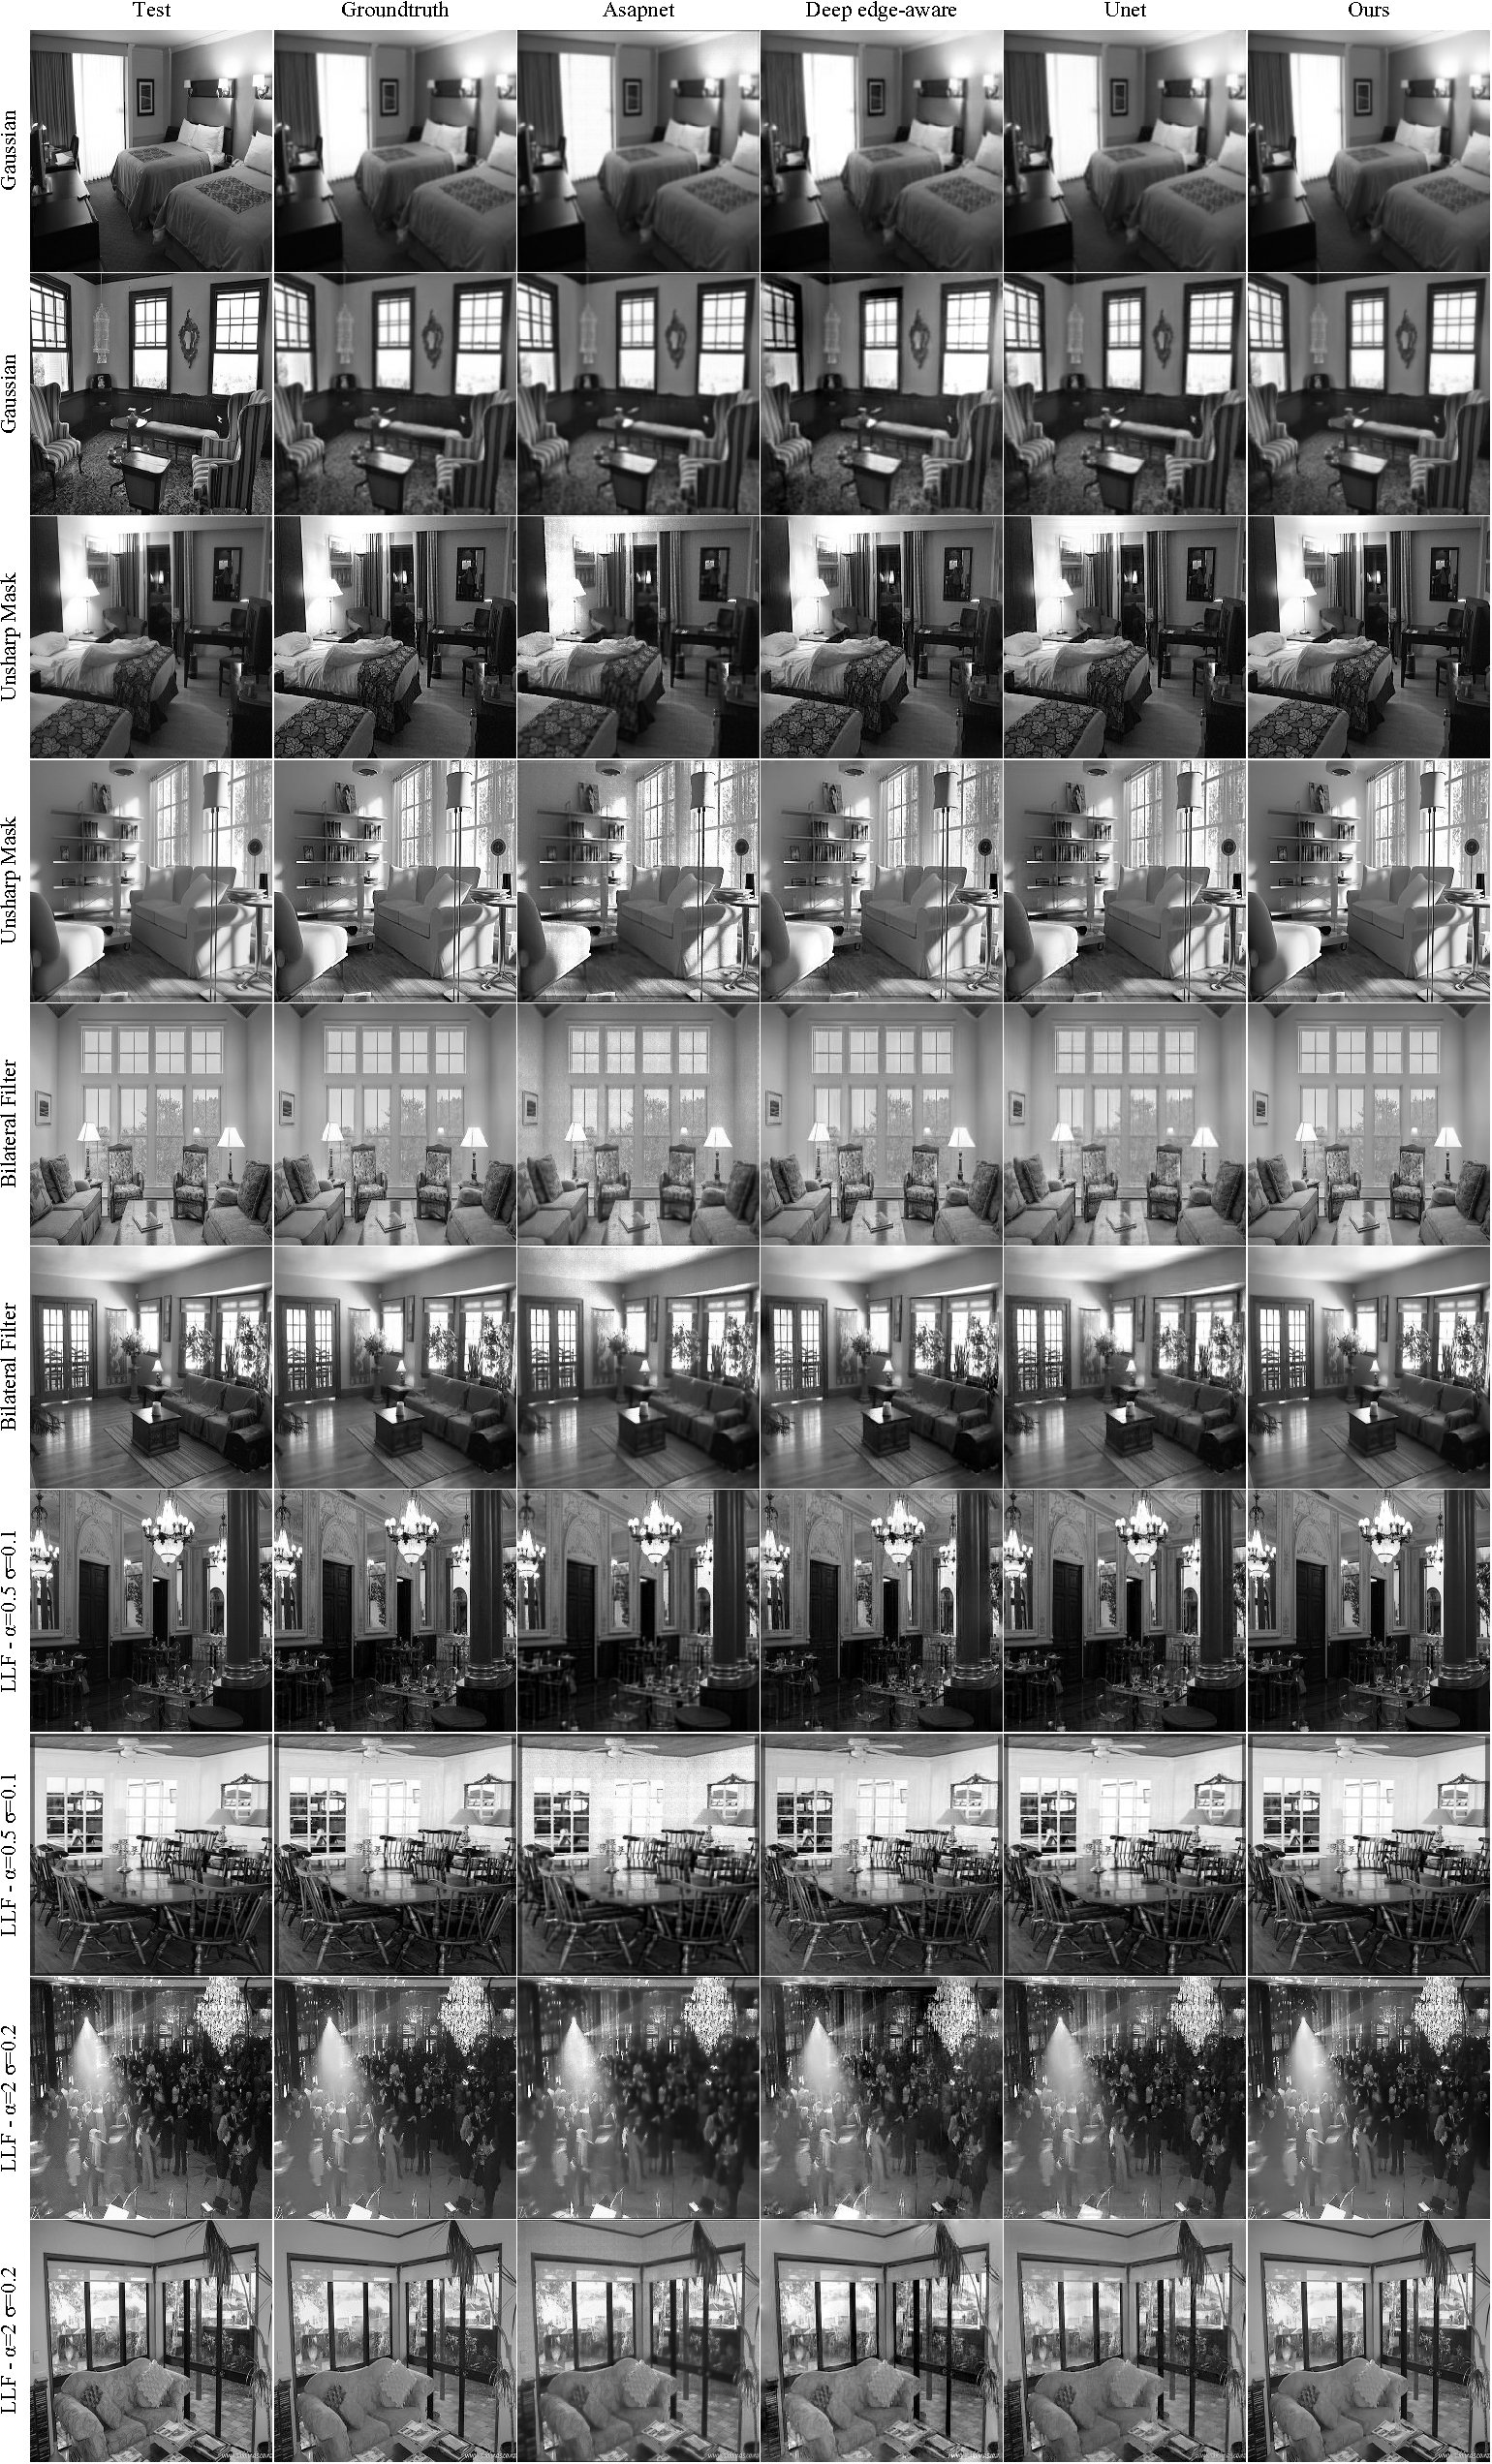
\includegraphics[width=0.8\linewidth]{Chapters/appendix-figs/room.pdf}}

   \caption{Qualitative comparison - Additional results.}
   \label{fig:appendix-DR-room}
\end{figure}


\begin{figure}[ht]
  \centering
  % \fbox{\rule{0pt}{2in} \rule{0.9\linewidth}{0pt}}
   % \adjustbox{trim={0.0\width} {.62\height} {0.0\width} {0.0\height},clip}%
  {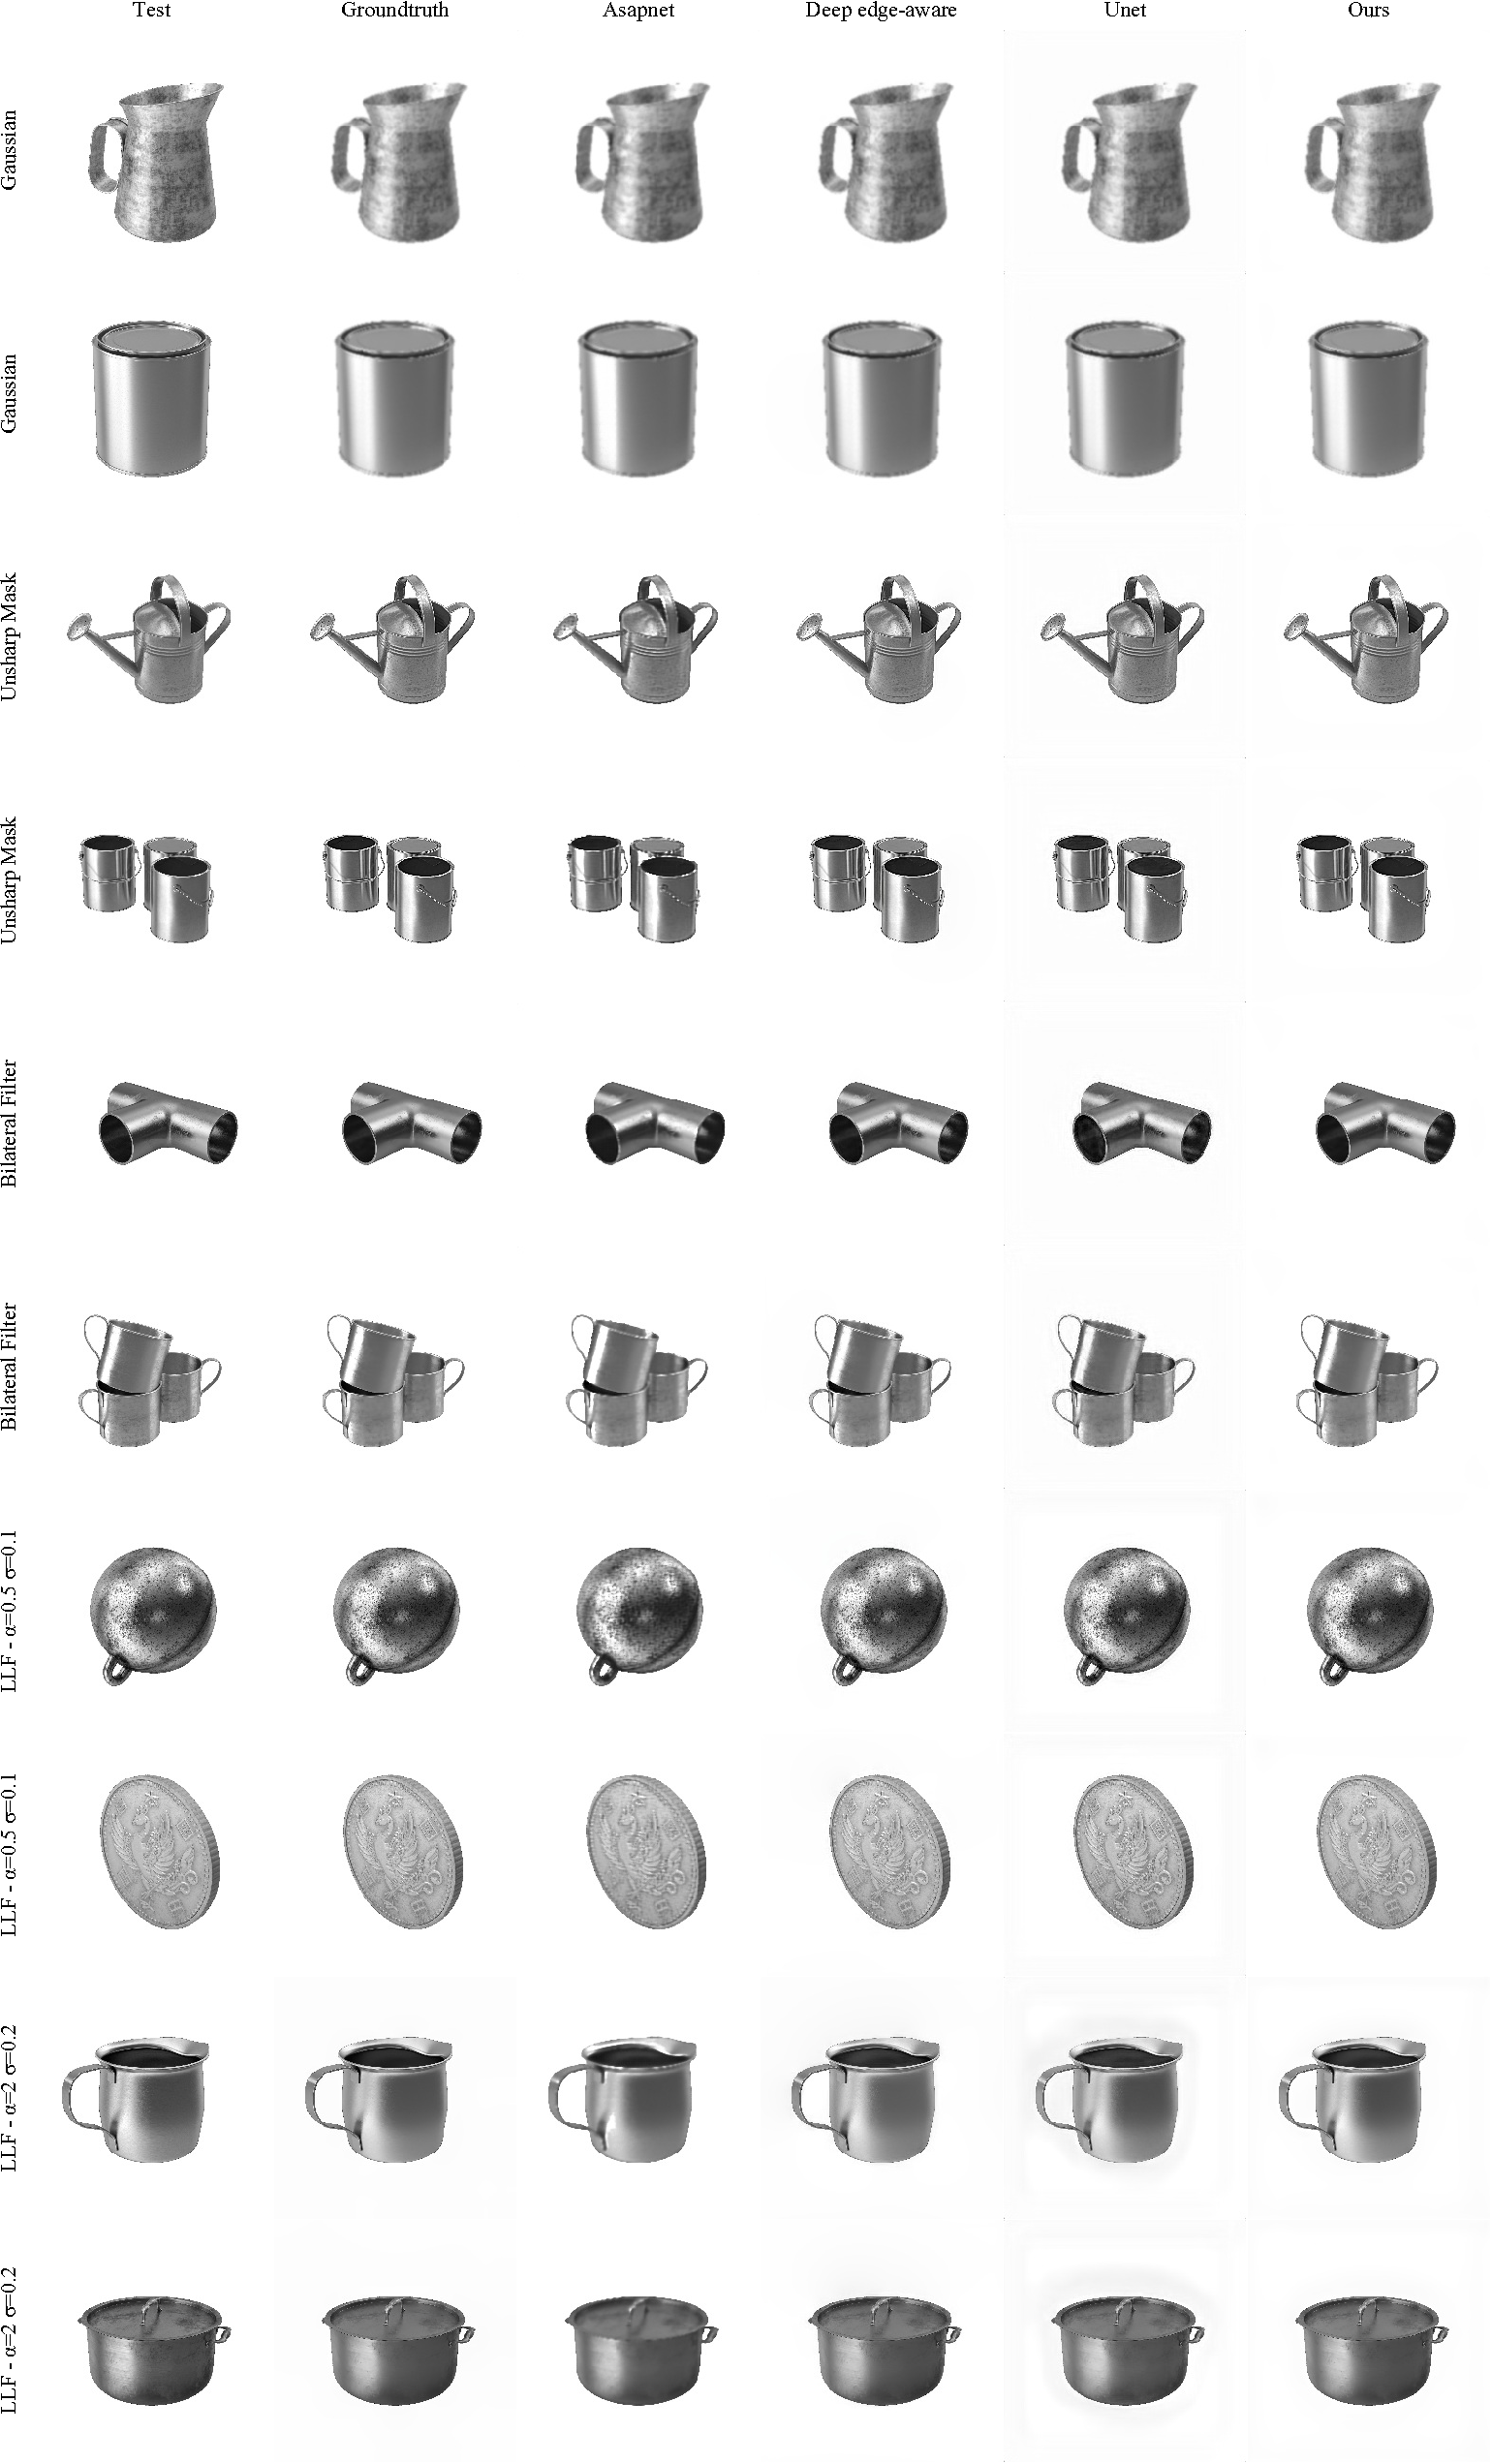
\includegraphics[width=0.8\linewidth]{Chapters/appendix-figs/material.pdf}}

   \caption{Qualitative comparison - Additional results.}
   \label{fig:appendix-DR-material}
\end{figure}

\begin{figure}[ht]
  \centering
  % \fbox{\rule{0pt}{2in} \rule{0.9\linewidth}{0pt}}

    %\adjustbox{trim={0.0\width} {.\height} {0.0\width} {0.385\height},clip}%
  {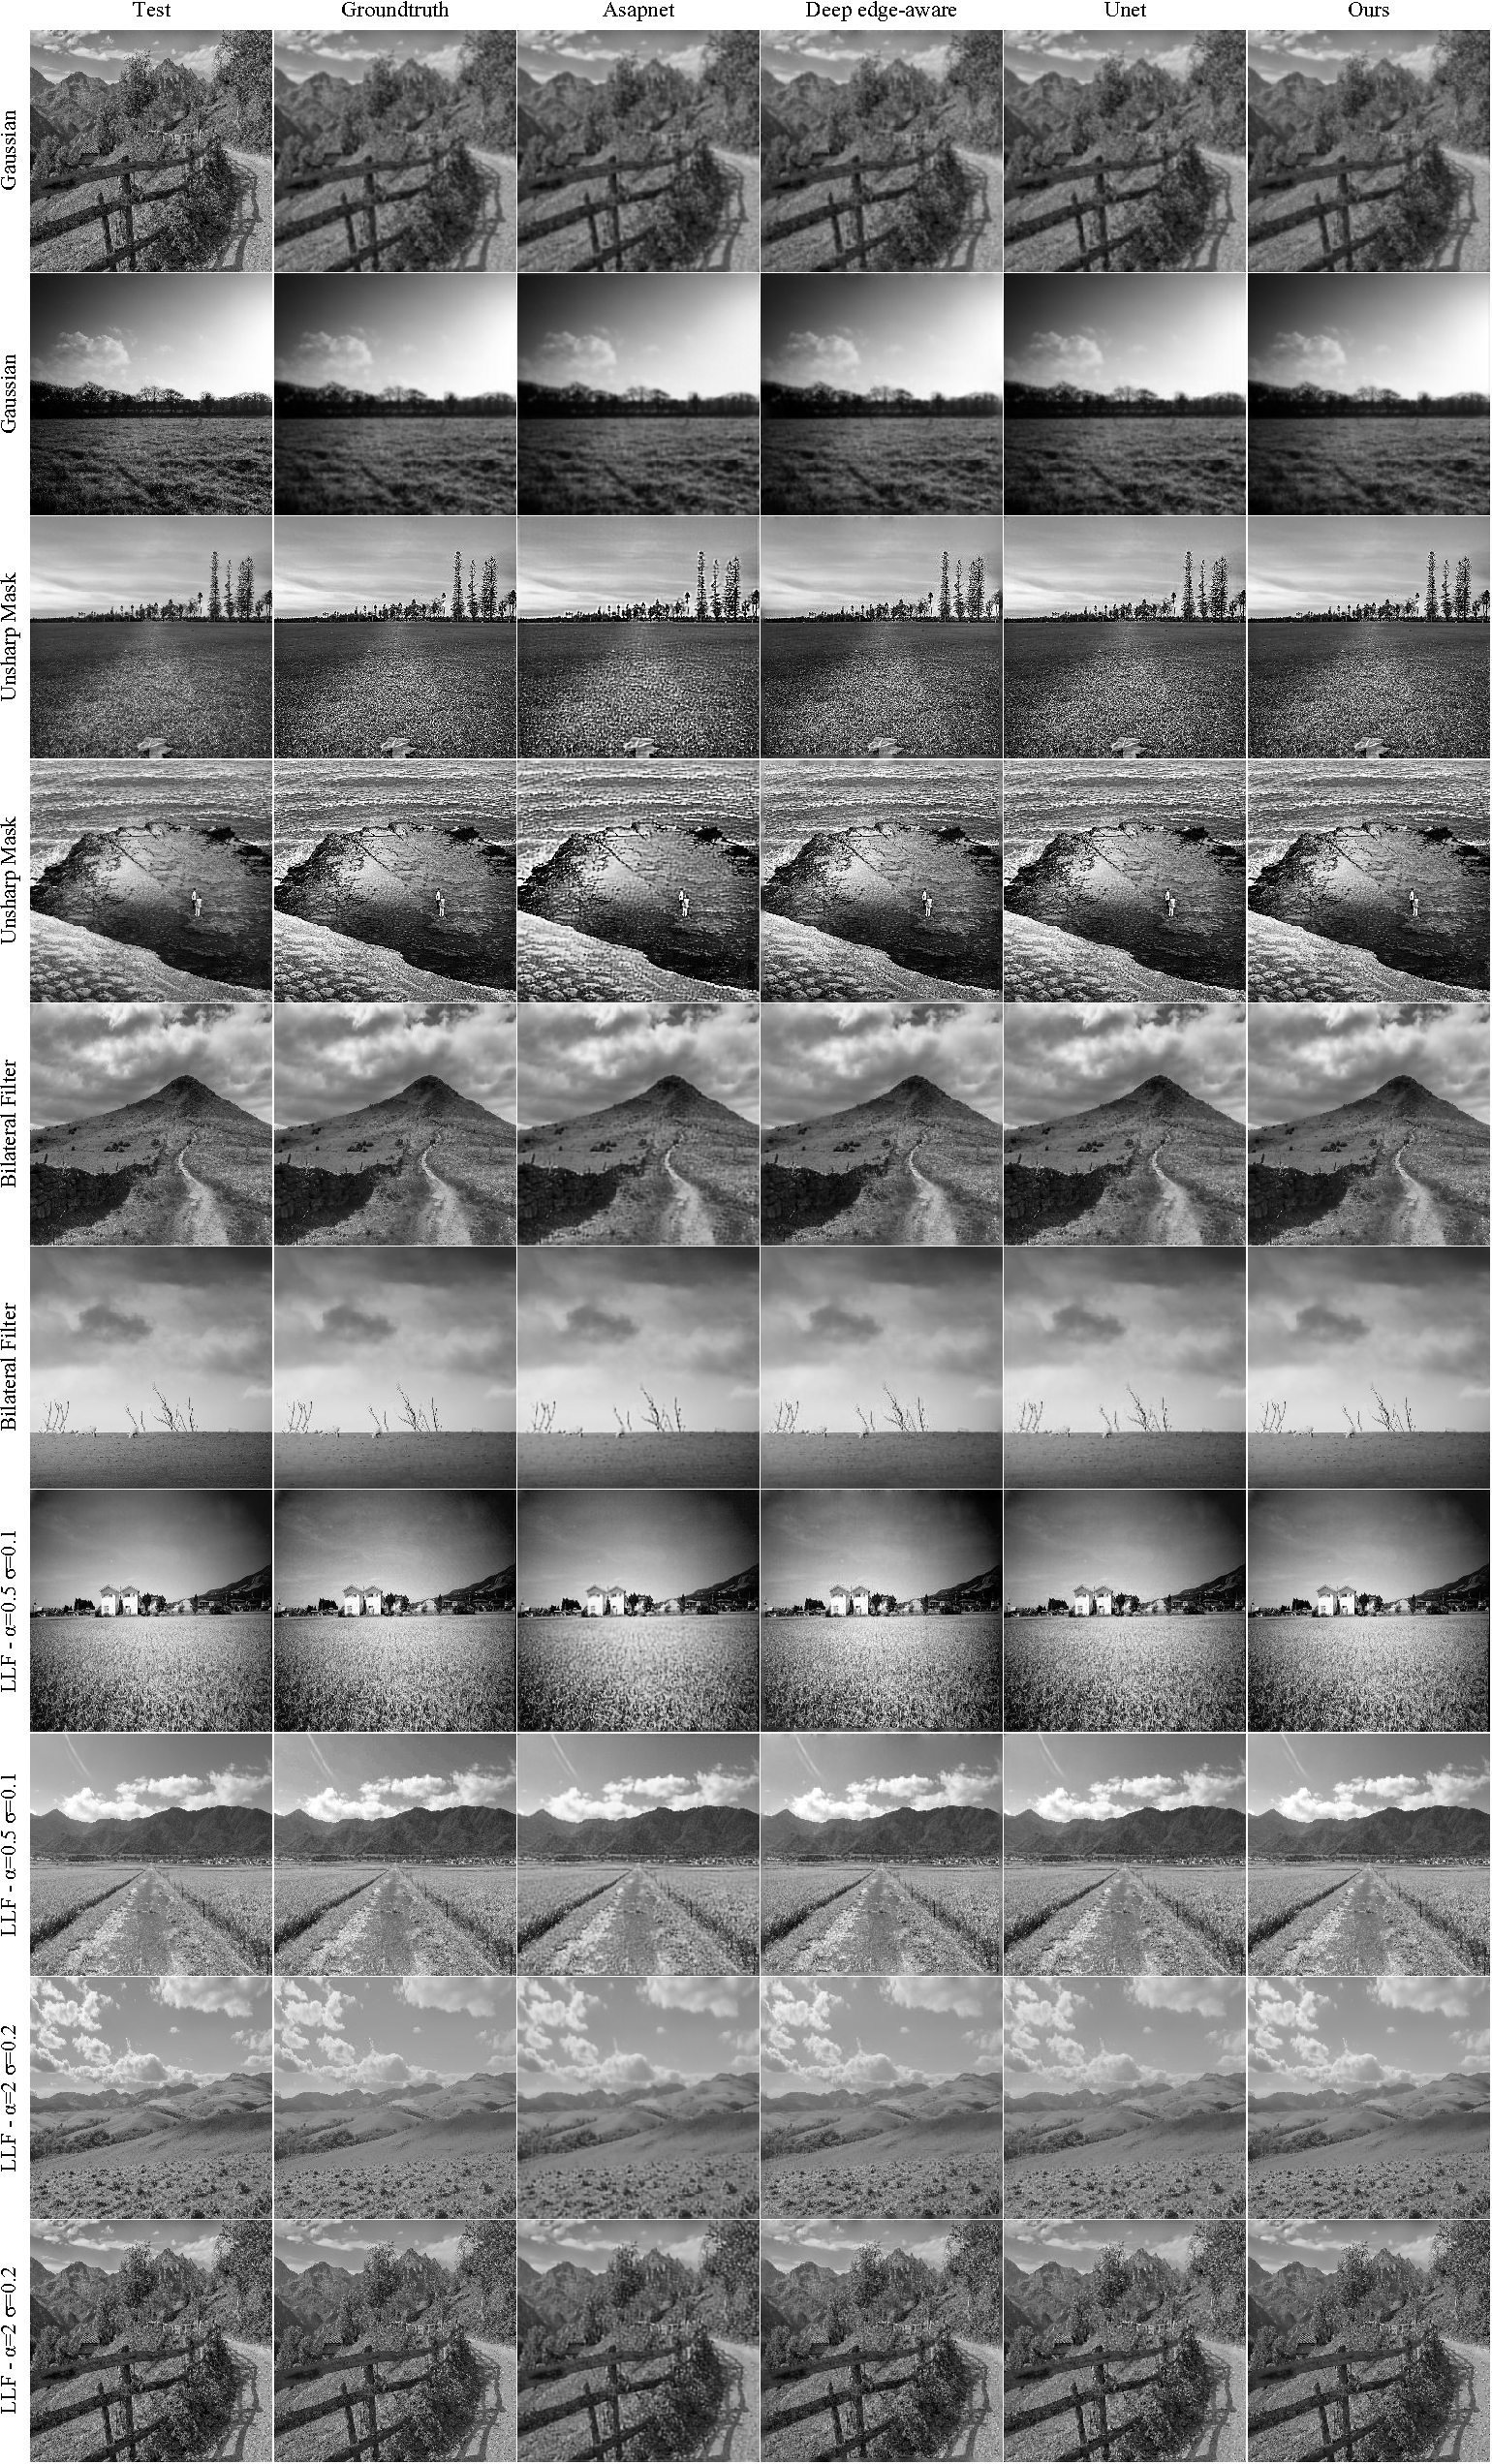
\includegraphics[width=0.8\linewidth]{Chapters/appendix-figs/landscape.pdf}}

   \caption{Qualitative comparison - Additional results.}
   \label{fig:appendix-DR-landscape}
\end{figure}

